\begin{center}
  \Large\textbf{BIOGRAFI PENULIS}
\end{center}
\vspace{2ex}

\addcontentsline{toc}{chapter}{BIOGRAFI PENULIS}

\begin{wrapfigure}{L}{0.3\textwidth}
  \centering
  \vspace{-3ex}
  % Ubah nama file gambar berikut dengan nama file foto dari mahasiswa pertama
  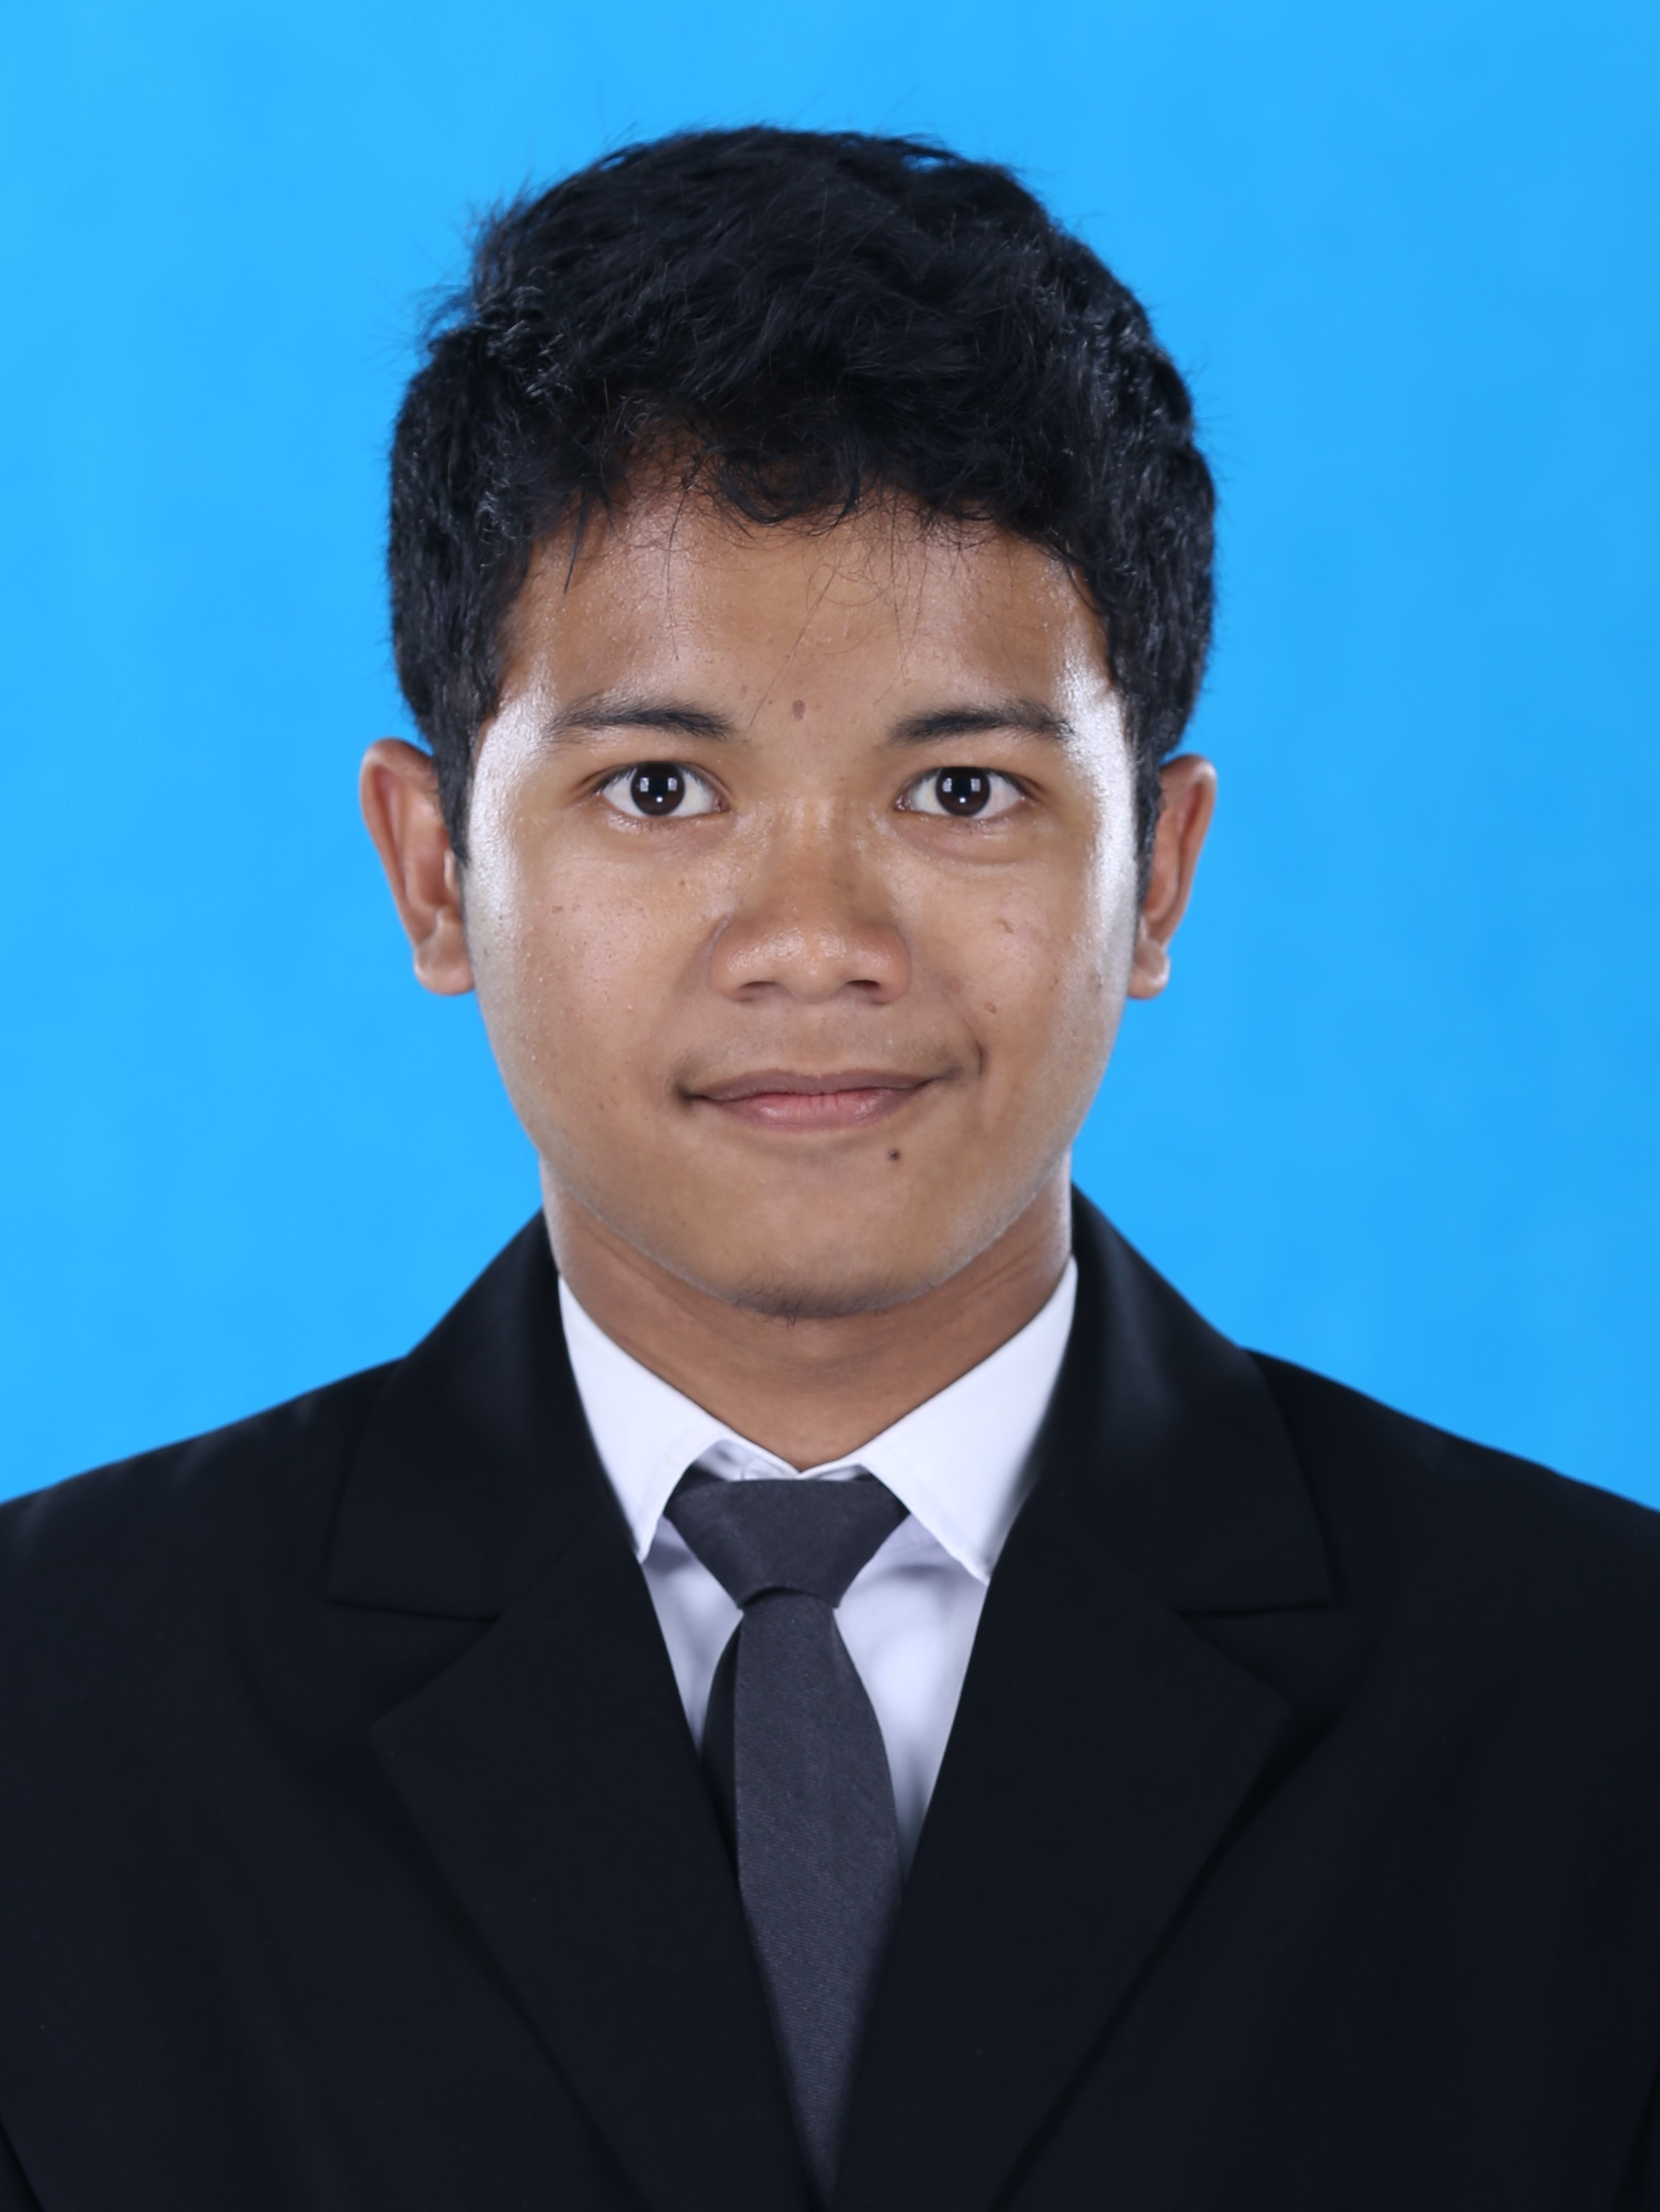
\includegraphics[width=0.3\textwidth]{gambar/ynw.jpg}
  \vspace{-4ex}
\end{wrapfigure}

% Ubah kalimat berikut dengan biografi dari mahasiswa pertama
\noindent Yusuf Nur Wahid, biasa dipanggil Ucup oleh teman-temannya lahir pada tanggal 18 Oktober 1998 di Banyuwangi.
Penulis memiliki riwayat pendidikan SDN 1 Cluring, SMPN 1 Cluring, SMAN 1 Genteng, dan S1 Teknik Komputer di ITS.
Selama kuliah penulis sempat menjadi asisten laboratorium \textbf{B201 Telematika} ITS pada periode 2019-2021.
Penulis juga memiliki hobi menulis kode karena menulis kode baginya adalah hal yang menyenangkan.
Apabila pembaca memiliki saran, kritik, ataupun pertanyaan mengenai laporan magang ini dapat menghubungi penulis melalui \textit{email} \href{mailto:yusufedu@gmail.com}{yusufedu@gmail.com}.
\begin{comment}
\vspace{2ex}

\begin{wrapfigure}{L}{0.3\textwidth}
  \centering
  \vspace{-3ex}
  % Ubah nama file gambar berikut dengan nama file foto dari mahasiswa kedua
  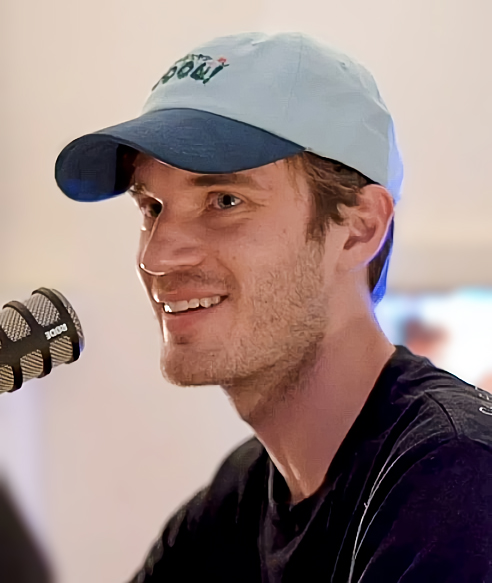
\includegraphics[width=0.3\textwidth]{gambar/felix.jpg}
  \vspace{-4ex}
\end{wrapfigure}

% Ubah kalimat berikut dengan biografi dari mahasiswa kedua
\noindent Felix Arvid Ulf Kjellberg, lahir pada \lipsum[2] ///
\end{comment}